\documentclass[12pt]{report}
\usepackage[utf8]{inputenc}
\usepackage[margin=1.2in]{geometry}
\usepackage{graphicx}
\usepackage{float}
\usepackage{subcaption}
\usepackage{amsmath}
\usepackage{amssymb}
\usepackage{ulem}
\usepackage{bm}
\usepackage{framed}
\usepackage{xcolor}
\usepackage{ragged2e}
\usepackage{color}
\usepackage{soul}
\usepackage{cancel}
\graphicspath{ {images/} }
\setlength{\parskip}{1em}
\allowdisplaybreaks


\usepackage{titling}
\newcommand{\subtitle}[1]{%
	\posttitle{%
		\par\end{center}
	\begin{center}\large#1\end{center}
	\vskip0.5em}%
}

\newenvironment{blueframed}[1][blue]
{\def\FrameCommand{\fboxsep=\FrameSep\fcolorbox{#1}{white}}%
\MakeFramed {\advance\hsize-\width \FrameRestore}}
{\endMakeFramed}

\newenvironment{spmatrix}[1]
{\def\mysubscript{#1}\mathop\bgroup\begin{bmatrix}}
{\end{bmatrix}\egroup_{\textstyle\mathstrut\mysubscript}}


\title{Tutorial 4}
\author{Quang Bui}
\subtitle
{
	\textbf{keywords}: matrix, matrices, vector, column space, histogram, scatter plot, mean, standard deviation, regression, simple, conditional expectation, OLS estimator, prediction, R squared, residual, interpretation, intercept, slope 
	
	\textbf{estimated reading time}: 35 minutes
}
\date{August 14, 2018}

\begin{document}
	
\maketitle

\section*{Question 1}
\textcolor{red}{\underline{Matrix multiplication}}

\noindent \textcolor{red}{Show that post-multiplying a matrix by a vector produces a linear combination of the columns of the matrix weighted by the elements of the vector.}

\justify
\begin{blueframed}
\textcolor{blue}{\textbf{Background}}
\vspace{-\baselineskip}
\justify
\textcolor{blue}{If \textbf{\textit{M}} and \textbf{\textit{N}} are matrices/vectors then the matrix multiplication, \textbf{\textit{MN}}, is only computable if the number of columns in \textit{M} equals to the number of rows in \textbf{\textit{N}}.}

\noindent \textcolor{blue}{Suppose that \textbf{\textit{M}} and \textbf{\textit{N}} are given by,}
\textcolor{blue}
	{$$\underset{2\times2}{\textbf{\textit{M}}}
		=
		\begin{bmatrix}
			a & b \\
			c & d 
		\end{bmatrix}
	$$}
\textcolor{blue}
	{$$\underset{2\times1}{\textbf{\textit{N}}}
		=
		\begin{bmatrix}
			e \\
			f  
	\end{bmatrix}
	$$}

\noindent \textcolor{blue}{Since the number of columns in \textbf{\textit{M}} equals to the number of rows in \textbf{\textit{N}}, \textbf{\textit{MN}} is computable.}

\noindent \textcolor{blue}{To compute \textbf{\textit{MN}},}
\textcolor{blue}
{$$\underset{2\times1}{\textbf{\textit{MN}}}
	=
	\begin{bmatrix}
	a & b \\
	c & d 
	\end{bmatrix}
	\begin{bmatrix}
	e \\
	f 
	\end{bmatrix}
	=
	\begin{bmatrix}
	ae+bf \\
	ce+df
	\end{bmatrix}
$$}
\end{blueframed}

\justify
Post-multiple matrix \textbf{\textit{X}} by vector $\widehat{\boldsymbol{\beta}}$,
{$$\underset{4\times2}{\textbf{\textit{X}}}
	=
	\begin{bmatrix}
	1 & 3 \\
	1 & 2 \\
	1 & 2 \\
	1 & 1 
	\end{bmatrix}
$$}
{$$\underset{2\times1}{\widehat{\boldsymbol{\beta}}}
	=
	\begin{bmatrix}
	0.7 \\
	0.2 
	\end{bmatrix}
$$}
{$${\textbf{\textit{X}}\widehat{\boldsymbol{\beta}}}
	=
	?
$$}
\justify 
Let $\widehat{\textbf{\textit{y}}}=\textbf{\textit{X}}\widehat{\boldsymbol{\beta}}$
{$$\underset{4\times1}{\widehat{\textbf{\textit{y}}}}
	=
	\underset{4\times1}{\textbf{\textit{X}}\widehat{\boldsymbol{\beta}}}
	=
	\begin{bmatrix}
	1 & 3 \\
	1 & 2 \\
	1 & 2 \\
	1 & 1 
	\end{bmatrix}
	\begin{bmatrix}
	0.7 \\
	0.2 
	\end{bmatrix}
$$}
\justify 
Since the no. of columns in \textbf{\textit{X}} equals to the no. of rows in $\widehat{\boldsymbol{\beta}}$, $\widehat{\textbf{\textit{y}}}$ is computable
{$$\underset{4\times1}{\widehat{\textbf{\textit{y}}}}
	=
	\begin{bmatrix}
	1 & 3 \\
	1 & 2 \\
	1 & 2 \\
	1 & 1 
	\end{bmatrix}
	\begin{bmatrix}
	0.7 \\
	0.2 
	\end{bmatrix}
	=
$$}
\justify
By factoring out the constants, $0.7$ and $0.2$, we can see that $\widehat{\textbf{\textit{y}}}$ is a linear combination of the columns of \textbf{\textit{X}}, weighted by $0.7$ and $0.2$,
{$$\underset{4\times1}{\widehat{\textbf{\textit{y}}}}
	=	
$$}

\newpage
\section*{Question 2}
\textcolor{red}{\underline{Generalising results from Question 1}}

\noindent \textcolor{red}{Generalise the result from Question 1 for the case of $n$ observations an \textbf{\textit{X}} matrix of 3 columns and a $\widehat{\boldsymbol{\beta}}$ vector of 3 rows.}
\begin{align*}
	\underset{n\times3}{\textbf{\textit{X}}}
	&=
	\begin{bmatrix}
	x_{11} & x_{12} & x_{13} \\
	x_{21} & x_{22} & x_{23} \\
	\vdots & \vdots & \vdots \\
	x_{n1} & x_{n2} & x_{n3} 
	\end{bmatrix} \\
	\underset{3\times1}{\widehat{\boldsymbol{\beta}}}
	&=
	\begin{bmatrix}
	\hat{\beta}_1 \\
	\hat{\beta}_2 \\
	\hat{\beta}_3 
	\end{bmatrix} \\
	\widehat{\textbf{\textit{y}}}
	&=
	{\textbf{\textit{X}}\widehat{\boldsymbol{\beta}}}
	=\ ?
\end{align*}
\justify 
Again, we can show that the linear combination of the columns of \textbf{\textit{X}} equals to the sum of each column of \textbf{\textit{X}} weighted/multiplied by each corresponding element in $\widehat{\boldsymbol{\beta}}$,
\begin{align*}
\widehat{\textbf{\textit{y}}} &=\ 1^{st}\ column\ of\ \textbf{\textit{X}} \times\ 1^{st}\ element\ of\ \widehat{\boldsymbol{\beta}} \\
&+\ 2^{nd}\ column\ of\ \textbf{\textit{X}} \times\ 2^{nd}\ element\ of\ \widehat{\boldsymbol{\beta}}\\
&+\ 3^{rd}\ column\ of\ \textbf{\textit{X}} \times\ 3^{rd}\ element\ of\ \widehat{\boldsymbol{\beta}} \\
\underset{n\times1}{\widehat{\textbf{\textit{y}}}}
&=
\begin{bmatrix}
x_{11} & x_{12} & x_{13} \\
x_{21} & x_{22} & x_{23} \\
\vdots & \vdots & \vdots \\
x_{n1} & x_{n2} & x_{n3} 
\end{bmatrix}
\begin{bmatrix}
\hat{\beta}_1 \\
\hat{\beta}_2 \\
\hat{\beta}_3 
\end{bmatrix} \\
&=
\begin{bmatrix}
x_{11}\hat{\beta}_1+x_{12}\hat{\beta}_2+	x_{13}\hat{\beta}_3 \\
x_{21}\hat{\beta}_1+x_{22}\hat{\beta}_2+	x_{23}\hat{\beta}_3 \\
\vdots \\
x_{n1}\hat{\beta}_1+x_{n2}\hat{\beta}_2+	x_{n3}\hat{\beta}_3 
\end{bmatrix} \\
&=
\begin{bmatrix}
x_{11}\hat{\beta}_1 \\
x_{21}\hat{\beta}_1 \\
\vdots \\
x_{n1}\hat{\beta}_1 
\end{bmatrix}
+
\begin{bmatrix}
x_{12}\hat{\beta}_2 \\
x_{22}\hat{\beta}_2 \\
\vdots \\
x_{n2}\hat{\beta}_2 
\end{bmatrix}
+
\begin{bmatrix}
x_{13}\hat{\beta}_3 \\
x_{23}\hat{\beta}_3 \\
\vdots \\
x_{n3}\hat{\beta}_3 
\end{bmatrix} \\
&=
\begin{bmatrix}
x_{11} \\
x_{21} \\
\vdots \\
x_{n1} 
\end{bmatrix}
\hat{\beta}_1
+
\begin{bmatrix}
x_{12} \\
x_{22} \\
\vdots \\
x_{n2} 
\end{bmatrix}
\hat{\beta}_2
+
\begin{bmatrix}
x_{13} \\
x_{23} \\
\vdots \\
x_{n3} 
\end{bmatrix}
\hat{\beta}_3
\end{align*}

\newpage
\section*{Question 3}
\noindent \textcolor{red}{This question is based on question C4 of the textbook. It is based on data on monthly salary and other characteristics of a random sample of 935 individuals. These data are in the file $wage2.wf1$. We concentrate on $wage$ as the dependent variable and the $IQ$ as the independent variable.}

\noindent \textcolor{red}{\underline{Descriptive analytics - ``looking" at the data through summary measures}}

\noindent \textcolor{red}{Obtain a histogram and summary statistics for the variables $wage$ and $IQ$ and a scatter plot of $wage$ against $IQ$.}
\begin{center}
\noindent $\textbf{\textit{wage}}$ - \textbf{monthly earnings (\$)}
\end{center}
\noindent To obtain the histogram of the $wage$ in EViews,
$$1.\ Double\ click\ on\ wage\ from\ the\ workfile$$
\begin{figure}[H]
\centering
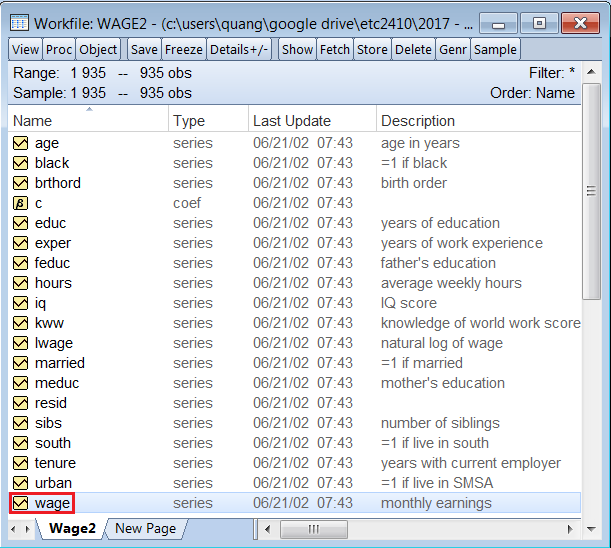
\includegraphics{q3_1}
\end{figure}
\vspace{-\baselineskip}
$$2.\ View \to Descriptive\ Statistics\ \&\ Tests \to Histograms\ and\ Stats$$
\begin{figure}[H]
\centering
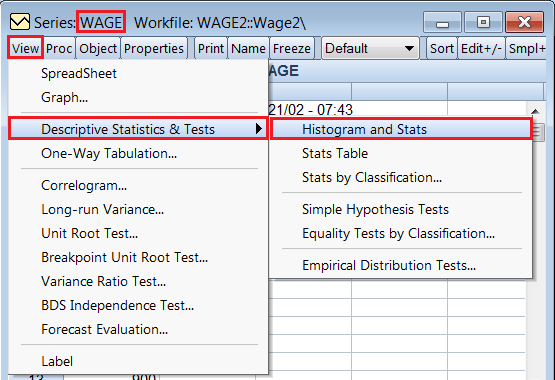
\includegraphics{q3_2}
\end{figure}
\vspace{-\baselineskip}
\begin{figure}[H]
\centerline{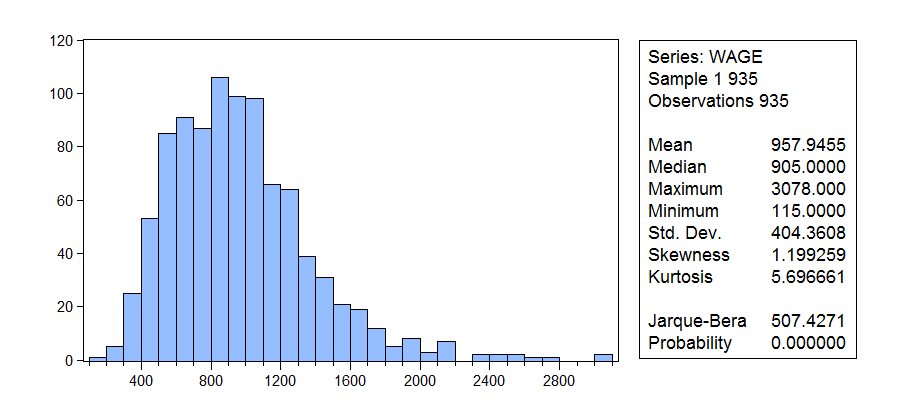
\includegraphics{q3_3}}
\caption{Histogram and descriptive statistics of monthly earnings (\$).}
\label{fig:hist1}
\end{figure}
\vspace{-\baselineskip}
\noindent As we can see from Figure \ref{fig:hist1}, monthly earnings is positively skewed (right-tailed) with mean and median monthly earnings of \$957.95 and \$905.00 respectively. \par
\begin{center}
$\textbf{\textit{IQ}}$ - \textbf{IQ score}
\end{center}
\noindent To obtain the histogram of the $IQ$ in EViews,
$$1.\ Double\ click\ on\ IQ\ from\ the\ workfile$$
\begin{figure}[H]
	\centering
	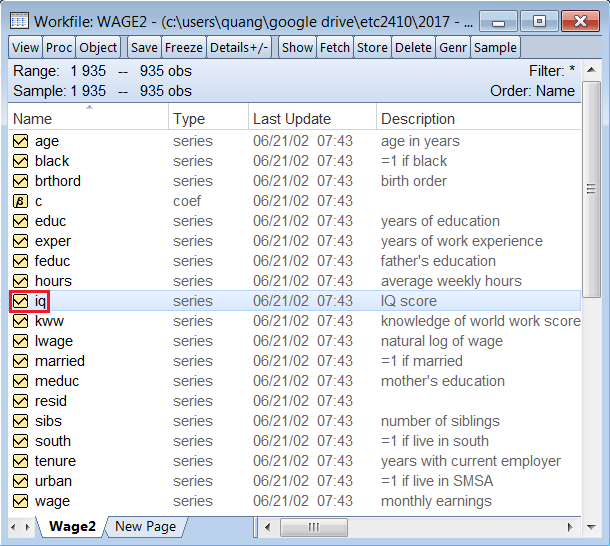
\includegraphics{q3_4}
\end{figure}
\vspace{-\baselineskip}
$$2.\ View \to Descriptive\ Statistics\ \&\ Tests \to Histograms\ and\ Stats$$
\begin{figure}[H]
	\centering
	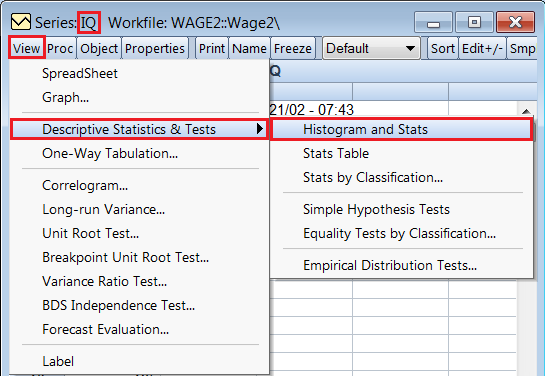
\includegraphics{q3_5}
\end{figure}
\vspace{-\baselineskip}
\begin{figure}[H]
	\centerline{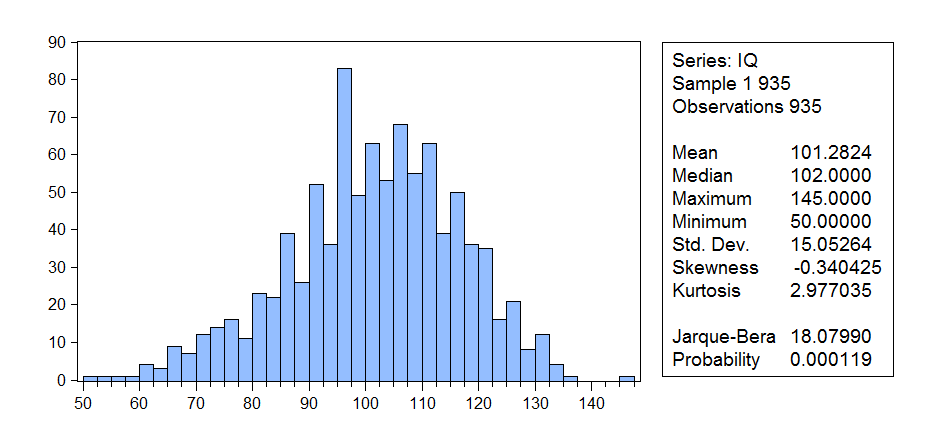
\includegraphics{q3_6}}
	\caption{Histogram and descriptive statistics of IQ score.}
	\label{fig:hist2}
\end{figure}
\vspace{-\baselineskip}
\noindent As we can see from Figure \ref{fig:hist2}, IQ score is very slightly negatively skewed (left-tailed) with mean and median IQ score of \$101.28 and \$102 respectively (almost symmetrical). \par
\noindent Theoretically, IQ score is normally distributed with the population parameters,
$$population\ mean = \mu = 100$$
$$population\ standard\ deviation = \sigma = 15$$
\noindent From the empirical rule, it follows that 68\%, 95\%, and 99.7\% of individuals have an IQ score within 1, 2, and 3 standard deviations of the mean respectively,
$$68\%: IQ\ score\ [85,115]$$
$$95\%: IQ\ score\ [70,130]$$
$$99.7\%: IQ\ score\ [55,145]$$
\noindent The sample mean and standard deviation are ‘close’ to their population counterpart,
$$sample\ mean = \hat{\mu} = \overline{IQ} = 101.28$$
$$sample\ standard\ deviation = \hat{\sigma} = 15.05$$
\noindent There is one outlier with an IQ score of 145 (theoretically, this individual is 3 population standard deviations above the population mean).
\begin{center}
	\noindent \textbf{Scatter plot of \textit{wage} against \textit{IQ}}
\end{center}
\noindent The dependent variable goes on the y-axis and the independent variable goes on the x-axis of a scatter plot. Since $wage$ is the dependent variable it goes in the y-axis and $IQ$ is the independent variable so it goes in the x-axis.

\noindent To obtain a scatter plot of $wage$ against $IQ$,
$$1.\ Quick \to Graph \dots$$
\begin{figure}[H]
	\centering
	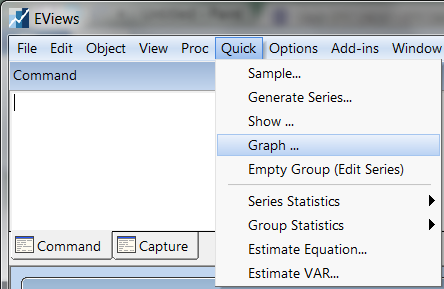
\includegraphics{q3_7}
\end{figure}
\vspace{-\baselineskip}
$$2.\ Series\ List:\ iq\ wage$$
$$(x-variable\ first\ then\ y-variable)$$
\begin{figure}[H]
	\centering
	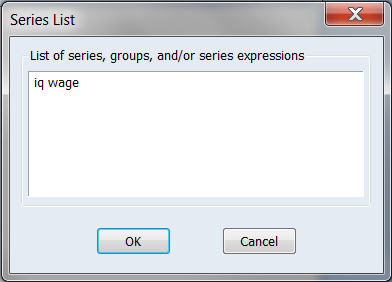
\includegraphics{q3_8}
\end{figure}
\vspace{-\baselineskip}
$$3.\ Specific:\ Scatter \to Fit\ Lines:\ Regression\ Line$$
\begin{figure}[H]
	\centering
	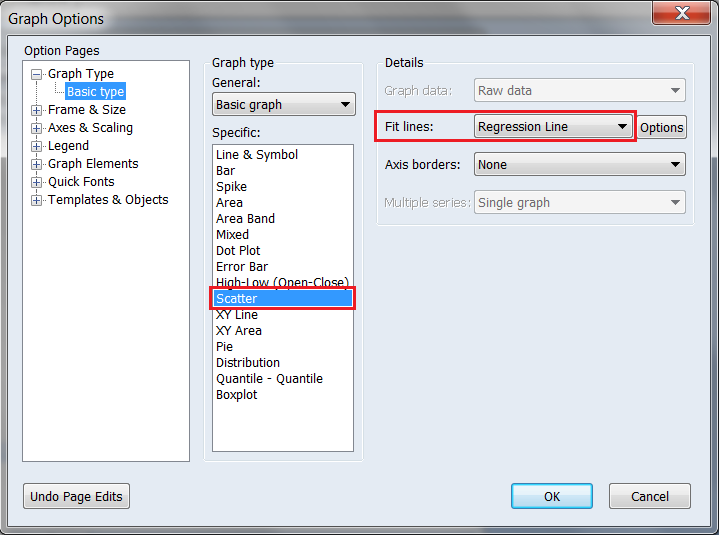
\includegraphics{q3_9}
\end{figure}
\vspace{-\baselineskip}
\begin{figure}[H]
	\centerline{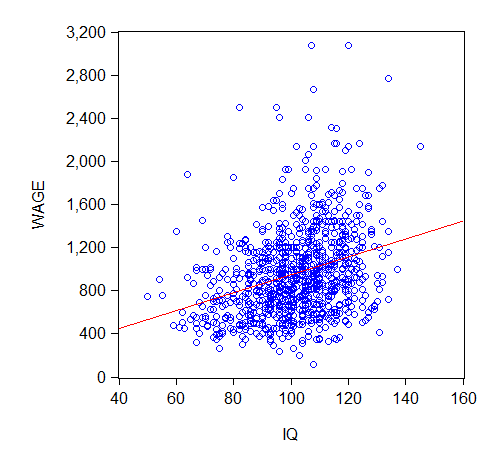
\includegraphics{q3_10}}
	\caption{Scatter plot of monthly earnings (\$) against IQ score.}
	\label{fig:scat1}
\end{figure}
\vspace{-\baselineskip}
\noindent Visual inspection of Figure \ref{fig:scat1} reveals that there is a positive relationship between IQ score and monthly earnings, however, this relationship does not appear to be linear. We also observe that the variability of monthly earnings increases as IQ score increases. \par
\noindent The red line through the scatter plot is a regression line of the estimated model,
$$\widehat{wage} = \hat{\beta}_0 + \hat{\beta}_2IQ$$

\noindent \textcolor{red}{\underline{(a) Simple Regression Model, Estimation, Interpretation of Slope Coefficient and $R^2$}}

\noindent \textcolor{red}{Estimate a simple regression model where a one-point increase in IQ score changes monthly earnings by a constant dollar amount.}
\justify
\begin{blueframed}
	\textcolor{blue}{\textbf{Background}}	
	\vspace{-\baselineskip}
	\justify
	\textcolor{blue}{\underline{Simple Linear Regression Model}}
	
	\noindent \textcolor{blue}{A \textit{simple} linear regression model has only one independent variable, $$y = \beta_0+\beta_1x_{1}+u$$ With a sample of \textit{n} observations, we can express this model in terms of each observation \textit{i},
	}
\end{blueframed}
\begin{blueframed}
	\noindent \textcolor{blue}
	{$$y_i = \beta_0+\beta_1x_{i1}+u_i \qquad i=1,2,\dots,n$$ or more compactly, in matrix notation
	$$\textbf{\textit{y}}=\textbf{\textit{X}}\boldsymbol{\beta}+\textbf{\textit{u}}$$
	where,
	$$
	\underset{n\times1}{\textbf{\textit{y}}}
	=
	\begin{bmatrix}
	y_{1} \\
	y_{2} \\
	\vdots \\
	y_{n} 
	\end{bmatrix}
	\quad
	\underset{n\times2}{\textbf{\textit{X}}}
	=
	\begin{bmatrix}
	1 & x_{11} \\
	1 & x_{21} \\
	\vdots & \vdots \\
	1 & x_{n1}  
	\end{bmatrix}
	\quad
	\underset{2\times1}{\boldsymbol{\beta}} =
	\begin{bmatrix}
	\beta_0 \\
	\beta_1 
	\end{bmatrix} 
	\quad
	\underset{n\times1}{\textbf{\textit{u}}}
	=
	\begin{bmatrix}
	u_{1} \\
	u_{2} \\
	\vdots \\
	u_{n} 
	\end{bmatrix} \\
	$$
	which gives,
	\begin{align*}
	\begin{bmatrix}
		y_{1} \\
		y_{2} \\
		\vdots \\
		y_{n} 
	\end{bmatrix}
	&=
	\begin{bmatrix}
	1 & x_{11} \\
	1 & x_{21} \\
	\vdots & \vdots \\
	1 & x_{n1}  
	\end{bmatrix}
	\begin{bmatrix}
	\beta_0 \\
	\beta_1
	\end{bmatrix}
	+
	\begin{bmatrix}
	u_{1} \\
	u_{2} \\
	\vdots \\
	u_{n} 
	\end{bmatrix} \\
	\begin{bmatrix}
	y_{1} \\
	y_{2} \\
	\vdots \\
	y_{n} 
	\end{bmatrix}
	&= 
	\begin{bmatrix}
	1 \\
	1 \\
	\vdots \\
	1   
	\end{bmatrix}
	\beta_0
	+
	\begin{bmatrix}
	x_{11} \\
	x_{21} \\
	\vdots \\
	x_{n1}   
	\end{bmatrix}
	\beta_1
	+
	\begin{bmatrix}
	u_{1} \\
	u_{2} \\
	\vdots \\
	u_{n} 
	\end{bmatrix}
	\end{align*}\\
	\uline{Multiple Linear Regression Model} \\ \\
	A \textit{multiple} linear regression model has more than one independent variable. For example, the following model contains 2 independent variables, $x_1$ and $x_2$,
	$$y = \beta_0+\beta_1x_{1}+\beta_2x_{2}+u$$
	As with the simple case, the multiple regression model can also be expressed in terms of each observation \textit{i},
	$$y_i = \beta_0+\beta_1x_{i1}+\beta_2x_{i2}+u_i \qquad i=1,2,\dots,n$$
	or in matrix notation,
	\begin{align*}
	\textbf{\textit{y}}&=\textbf{\textit{X}}\boldsymbol{\beta}+\textbf{\textit{u}} \\
	\begin{bmatrix}
	y_{1} \\
	y_{2} \\
	\vdots \\
	y_{n} 
	\end{bmatrix}
	&=
	\begin{bmatrix}
	1 & x_{11} & x_{12} \\
	1 & x_{21} & x_{22} \\
	\vdots & \vdots & \vdots \\
	1 & x_{n1} & x_{n2}  
	\end{bmatrix}
	\begin{bmatrix}
	\beta_0 \\
	\beta_1 \\
	\beta_2
	\end{bmatrix}
	+
	\begin{bmatrix}
	u_{1} \\
	u_{2} \\
	\vdots \\
	u_{n} 
	\end{bmatrix} \\
	\end{align*}
}
\end{blueframed}
\begin{blueframed}
	\textcolor{blue}{\begin{align*}
		\begin{bmatrix}
		y_{1} \\
		y_{2} \\
		\vdots \\
		y_{n} 
		\end{bmatrix}
		&= 
		\begin{bmatrix}
		1 \\
		1 \\
		\vdots \\
		1   
		\end{bmatrix}
		\beta_0
		+
		\begin{bmatrix}
		x_{11} \\
		x_{21} \\
		\vdots \\
		x_{n1}   
		\end{bmatrix}
		\beta_1
		+
		\begin{bmatrix}
		x_{12} \\
		x_{22} \\
		\vdots \\
		x_{n2}   
		\end{bmatrix}
		\beta_2
		+
		\begin{bmatrix}
		u_{1} \\
		u_{2} \\
		\vdots \\
		u_{n} 
		\end{bmatrix}
		\end{align*}
	}
\end{blueframed}
\noindent So a simple regression model where a one-point increase in IQ score changes wage by a constant amount is given by,
$$wage=\beta_0+\beta_1IQ+u$$
\noindent To estimate this model from the menu bar in EViews,
$$Quick \to Estimate\ Equation$$
\begin{figure}[H]
	\centering
	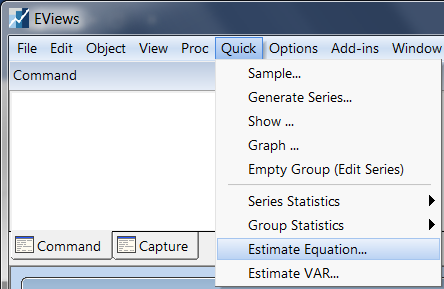
\includegraphics{q3_11}
\end{figure}
\vspace{-\baselineskip}
$$Equation\ Estimation: wage\ c\ iq$$
\begin{figure}[H]
	\centering
	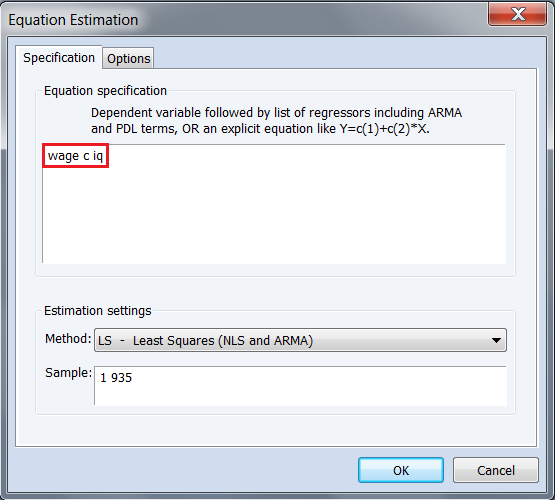
\includegraphics{q3_12}
\end{figure}
\vspace{-\baselineskip}
\noindent To estimate the model from the \textbf{Command window},
$$Command\ window: ls\ wage\ c\ iq$$
$$(press\ Enter\ to\ execute\ code)$$
\begin{figure}[H]
	\centering
	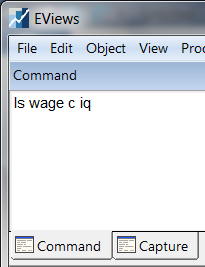
\includegraphics{q3_13}
\end{figure}
\vspace{-\baselineskip}
\noindent To name (save) the estimated equation,
$$Name \to Name\ to\ identify\ object: eq01$$
$$(This\ names\ the\ equation\ \textit{\textbf{eq01}})$$
\begin{figure}[H]
	\centering
	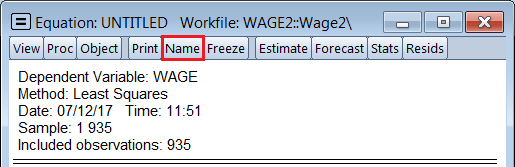
\includegraphics{q3_14}
\end{figure}
\vspace{-\baselineskip}
\begin{figure}[H]
	\centering
	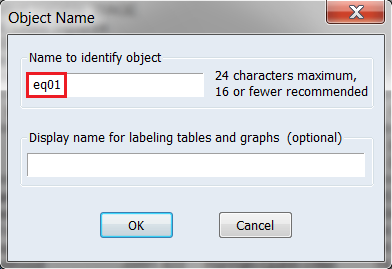
\includegraphics{q3_15}
\end{figure}
\vspace{-\baselineskip}
\noindent To save the residuals of this estimated model,
$$eq01 \to Proc \to Make\ Residual\ Series \dots \to Name\ of\ resid\ series: uhat01$$
$$(This\ names\ the\ equation\ \textit{\textbf{uhat01}})$$
\begin{figure}[H]
	\centering
	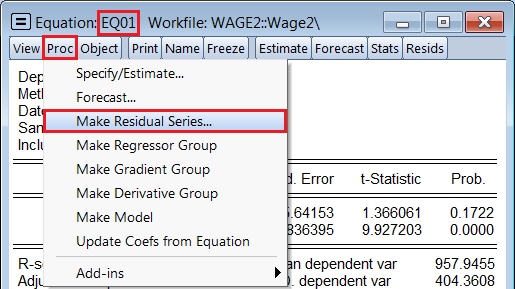
\includegraphics{q3_16}
\end{figure}
\vspace{-\baselineskip}
\begin{figure}[H]
	\centering
	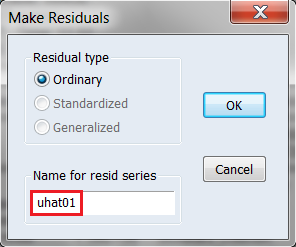
\includegraphics{q3_17}
\end{figure}
\vspace{-\baselineskip}
\noindent After clicking $OK$, the residuals should appears
\begin{figure}[H]
	\centering
	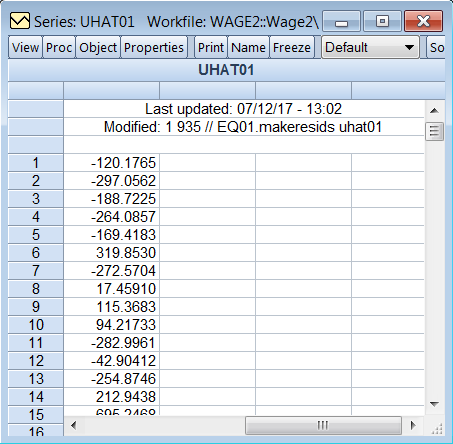
\includegraphics{q3_18}
\end{figure}
\vspace{-\baselineskip}
\newpage
\justify
\begin{blueframed}
	\textcolor{blue}{\textbf{Background}}
	\vspace{-\baselineskip}
	\justify
	\textcolor{blue}{\underline{Residuals}}
	
	\noindent \textcolor{blue}
	{
		Every estimated model comes with a set of residuals. The residuals from an estimated model is the difference between the actual value of $y$ and $\hat{y}$ (predicted $y$) for each observation $i$,
		$$\hat{u}_i = y_i-\hat{y}_i \qquad i=1,2,\dots,n$$
	}
	\textcolor{blue}
	{
		$$\hat{u}_1 = y_1-\hat{y}_1$$
		$$\hat{u}_2 = y_1-\hat{y}_2$$
		$$\vdots$$
		$$\hat{u}_n = y_n-\hat{y}_n$$
		For our estimated model of $wage$ on a constant and $IQ$ with a sample of 935 observations, $$\widehat{wage}_i = 116.9916+8.3031IQ_i \qquad i=1,2,\dots,935$$ the residuals are expressed as follows,
		$$\hat{u}_i = wage_i-\widehat{wage}_i \qquad i=1,2,\dots,935$$
		\begin{align*}
		\hat{u}_1 = wage_1&-\widehat{wage}_1 \\
		\hat{u}_2 = wage_2&-\widehat{wage}_2 \\
		&\ \vdots \\
		\hat{u}_{935} = wage_{935}&-\widehat{wage}_{935}
		\end{align*}
		Concretely,
		\begin{align*}
		wage_1-\widehat{wage}_1 &= wage_1 - (116.9916+8.3031IQ_1) \\
		&= 769-(116.9916+8.3031\times93) \\
		&= -120.18 \\
		wage_2-\widehat{wage}_2 &= wage_2 - (116.9916+8.3031IQ_2) \\
		&= 808-(116.9916+8.3031\times119) \\
		&= -297.05 \\
		&\ \vdots \\
		wage_{935}-\widehat{wage}_{935} &= wage_{935} - (116.9916+8.3031IQ_{935}) \\
		&= 1000-(116.9916+8.3031\times107) \\
		&= -5.42 
		\end{align*}
	}
\end{blueframed}
\begin{blueframed}
\begin{figure}[H]
	\centering
	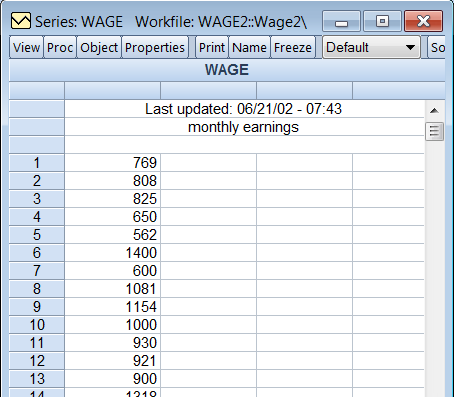
\includegraphics{q3_19}
	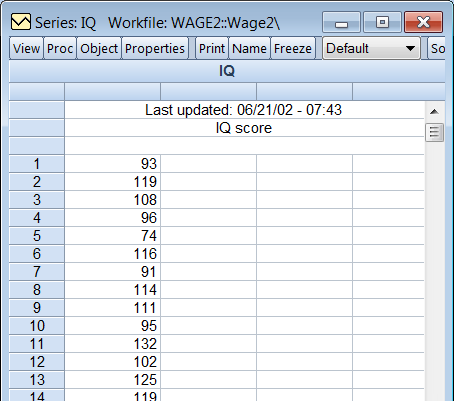
\includegraphics{q3_20}
\end{figure}
\vspace{-\baselineskip}
\end{blueframed}




%%%%%%%%%% TABLE OBJECT %%%%%%%%%%
\begin{table}[H]
	\centering
	\begin{tabular}{lrrrr}
		\multicolumn{3}{l}{Dependent Variable: WAGE}&\multicolumn{1}{c}{}&\multicolumn{1}{c}{}\\
		\multicolumn{3}{l}{Method: Least Squares}&\multicolumn{1}{c}{}&\multicolumn{1}{c}{}\\
		\multicolumn{2}{l}{Sample: 1 935}&\multicolumn{1}{c}{}&\multicolumn{1}{c}{}&\multicolumn{1}{c}{}\\
		\multicolumn{3}{l}{Included observations: 935}&\multicolumn{1}{c}{}&\multicolumn{1}{c}{}\\
		[4.5pt] \hline \\ [-4.5pt]
		\multicolumn{1}{c}{Variable}&\multicolumn{1}{r}{Coefficient}&\multicolumn{1}{r}{Std. Error}&\multicolumn{1}{r}{t-Statistic}&\multicolumn{1}{r}{Prob.}\\
		[4.5pt] \hline \\ [-4.5pt]
		\multicolumn{1}{c}{C}&\multicolumn{1}{r}{$116.9916$}&\multicolumn{1}{r}{$85.64153$}&\multicolumn{1}{r}{$1.366061$}&\multicolumn{1}{r}{$0.1722$}\\
		\multicolumn{1}{c}{IQ}&\multicolumn{1}{r}{$8.303064$}&\multicolumn{1}{r}{$0.836395$}&\multicolumn{1}{r}{$9.927203$}&\multicolumn{1}{r}{$0.0000$}\\
		[4.5pt] \hline \\ [-4.5pt]
		\multicolumn{1}{l}{R-squared}&\multicolumn{1}{r}{$0.095535$}&\multicolumn{2}{l}{Mean dependent var}&\multicolumn{1}{r}{$957.9455$}\\
		\multicolumn{1}{l}{Adjusted R-squared}&\multicolumn{1}{r}{$0.094566$}&\multicolumn{2}{l}{S.D. dependent var}&\multicolumn{1}{r}{$404.3608$}\\
		\multicolumn{1}{l}{S.E. of regression}&\multicolumn{1}{r}{$384.7667$}&\multicolumn{2}{l}{Akaike info criterion}&\multicolumn{1}{r}{$14.74529$}\\
		\multicolumn{1}{l}{Sum squared resid}&\multicolumn{1}{r}{$1.38E+08$}&\multicolumn{2}{l}{Schwarz criterion}&\multicolumn{1}{r}{$14.75564$}\\
		\multicolumn{1}{l}{Log likelihood}&\multicolumn{1}{r}{$-6891.422$}&\multicolumn{2}{l}{Hannan-Quinn criter.}&\multicolumn{1}{r}{$14.74924$}\\
		\multicolumn{1}{l}{F-statistic}&\multicolumn{1}{r}{$98.54936$}&\multicolumn{2}{l}{Durbin-Watson stat}&\multicolumn{1}{r}{$1.802114$}\\
		\multicolumn{1}{l}{Prob(F-statistic)}&\multicolumn{1}{r}{$0.000000$}&\multicolumn{1}{c}{}&\multicolumn{1}{c}{}&\multicolumn{1}{c}{}\\
		[4.5pt] \hline \\ [-4.5pt]
	\end{tabular}
	\caption{Regression output of $wage$ on a constant and $IQ$}
	\label{tbl:regout1}
\end{table}
\vspace{-\baselineskip}
\noindent When reporting the estimated model, we must not forget to include a `hat' above the dependent variable and report the standard error of $\hat{\beta}$ in parenthesis underneath its corresponding estimated coefficient,
$$\widehat{wage} = \underset{(85.6415)}{116.9916} + \underset{(0.8364)}{8.3031}IQ$$
\justify
\begin{blueframed}
	\textcolor{blue}{\textbf{Background}}
	\vspace{-\baselineskip}
	\justify
	\textcolor{blue}{\underline{Conditional Expectation}}
	
	\noindent \textcolor{blue}
	{
	Our simple regression model,
	$$wage = \beta_0+\beta_1IQ+u$$
	can also be written in terms of the expectation of $wage$ conditional on $IQ$,
	$$wage = E(wage|IQ)+u$$ 
	since,
	\begin{align*}
		E(wage|IQ) &= E(\beta_0+\beta_1IQ+u|IQ) \\
		&= E(\beta_0|IQ) + E(\beta_1IQ|IQ) + E(u|IQ) \\ 
		&= \beta_0 + \beta_1 IQ + 0 \\ &= \beta_0 + \beta_1 IQ
	\end{align*}}
\end{blueframed}
\begin{blueframed}
	\noindent \textcolor{blue}
	{
	$\beta_0$ and $\beta_1$ are the true but unknown population parameters in our model, which we wish to estimate using our sample data set. To estimate the simple regression model of $wage$ on a constant and $IQ$ is to effectively estimate the expected $wage$ conditional on $IQ$,
	\begin{align*}
		\widehat{wage} &= \hat{\beta}_0+\hat{\beta}_1IQ \\
		\widehat{E(wage|IQ)} &= \hat{\beta}_0+\hat{\beta}_1IQ
	\end{align*}
	$\hat{\beta}_0$ and $\hat{\beta}_1$ are estimators of $\beta_0$ and $\beta_1$ i.e. they are random variables which gives us estimates of $\beta_0$ and $\beta_1$ depending on the sample data set we feed it. \\ \\ But how does $\hat{\beta}_0$ and $\hat{\beta}_1$ estimate $\beta_0$ and $\beta_1$?
	}
	\justify
	\textcolor{blue}{\underline{OLS estimator}}

	\noindent \textcolor{blue}
	{
	Estimating the expected $wage$ conditional on $IQ$ involves estimating the unknown population parameters $\beta_0$ and $\beta_1$ and we do so by using the OLS estimator. The OLS estimator ‘finds’ or ‘chooses’ a value for $\hat{\beta}_0$ and $\hat{\beta}_1$ such that the sum of the squared differences between $wage$ and $\widehat{wage}$ for each observation $i$ in our sample,
	\begin{align*}
	&\sum_{i=1}^{n} (wage_i - \widehat{wage}_i)^2 \\
	%=&\sum_{i=1}^{n} (wage_i - \widehat{E(wage_i|IQ_i)})^2 \\
	=&\sum_{i=1}^{n} (wage_i - (\hat{\beta}_0+\hat{\beta}_1IQ_i))^2 \\
	=&\sum_{i=1}^{n} {\hat{u}_i}^2
	\end{align*}
	is as small as possible.
	Stated differently, the OLS estimator is a formula, $$\widehat{\boldsymbol{\beta}} =(\textbf{X}'\textbf{X})^{-1}\textbf{X}'\textbf{y}$$
	which after given some sample data, will find the values for $\hat{\beta}_0$ and $\hat{\beta}_1$ that minimises the sum of squared residuals. \\ \\
	For a simple linear regression model like $wage$, the OLS formula for $\hat{\beta}_0$ and $\hat{\beta}_1$ is given by, \begin{align*}
		\hat{\beta}_0 &= \overline{y} - \hat{\beta}_1 \overline{x} \\
		\hat{\beta}_1 &= \dfrac{\widehat{cov}(x_i , y_i)}{\widehat{var}(x_i)}
	\end{align*}
	}
\end{blueframed}
\begin{blueframed}
	\noindent \textcolor{blue}{Such that, $$\widehat{\boldsymbol{\beta}} =(\textbf{X}'\textbf{X})^{-1}\textbf{X}'\textbf{y}=\begin{bmatrix}
		\hat{\beta}_0 \\
		\hat{\beta}_1 
		\end{bmatrix} = \begin{bmatrix}
		\overline{y} - \hat{\beta}_1 \overline{x} \\
		\dfrac{\widehat{cov}(x_i , y_i)}{\widehat{var}(x_i)}
		\end{bmatrix}$$
	}
\end{blueframed}
\noindent \textcolor{red}{Find the predicted increase in $wage$ for an increase in $IQ$ of 15 points:}
$$\widehat{wage} = 116.9916+8.3031IQ$$
\noindent The model predicts/estimates that a 1-point increase in IQ score, increases monthly earnings by \$8.30 ($\hat{\beta}_1 = 8.30$), on average.
\noindent This implies that for a 15-point increase in IQ score, the model predicts monthly earnings to increase by 15 $\times$ \$8.3031 = \$124.55, on average.

\noindent \textcolor{red}{Does $IQ$ explain most of the variation in $wage$?}

\noindent From Table \ref{tbl:regout1}, $R^2 = 0.09554$. This means that the model explains 9.55\% of the variability in $wage$. Since this model contains only one independent variable, $IQ$, this implies that $IQ$ explains 9.55\% of the variability in $wage$ and 100-9.55\%=90.45\% is left unexplained by the model. (There is a lot of unexplained variation.)

\noindent \textcolor{red}{What is the relationship between the $R^2$ of this regression and the sample correlation coefficient between $wage$ and $IQ$?}
\begin{figure}[H]
	\centering
	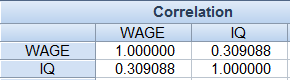
\includegraphics{q3_32}
\end{figure}
\vspace{-\baselineskip} 
$$R^2 = 0.0955$$
$$\widehat{corr}(wage,IQ) = 0.309088$$
$$(\widehat{corr}(wage,IQ))^2 = 0.309088^2 = 0.0955 = R^2$$
\noindent This relationship can only hold for a simple linear regression model.

\noindent \textcolor{red}{\underline{(b) Interpretation of the intercept coefficient}}

\noindent \textcolor{red}{What does the estimated intercept coefficient of,
$$\widehat{wage} = \underset{(85.6415)}{116.9916} + \underset{(0.8364)}{8.3031}IQ$$ mean?}
$$\hat{\beta}_0 = 116.9916$$
\noindent 	The model predicts that an individual with an IQ score of 0 will earn \$116.99 each month, on average. This interpretation is not meaningful because:
\begin{enumerate}
	\item Not possible for living person to have an IQ score of 0.
	\item We estimated our model with a sample of individuals with an IQ score between 50 (minimum) and 145 (maximum). Predictions based on values of the independent variable(s) outside of the range of values in the sample used to estimate the model should be avoided. Since $IQ = 0$ is outside this range, this interpretation is not meaningful.
\end{enumerate}
\noindent \textcolor{red}{Run a regression of $wage$ on a constant and $(IQ-100)$ and name this equation $eq02$ in EViews.}
$$wage = \alpha_0 + \alpha_1(IQ-100) + u$$
$$Quick \to Estimate\ Equation$$
\begin{figure}[H]
	\centering
	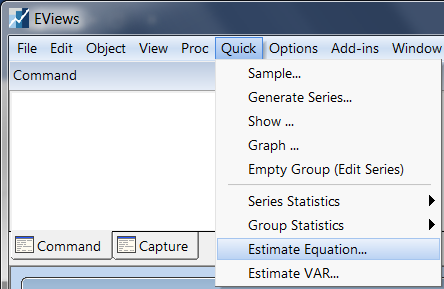
\includegraphics{q3_11}
\end{figure}
\vspace{-\baselineskip}
$$Equation\ Estimation: wage\ c\ iq-100$$
\begin{figure}[H]
	\centering
	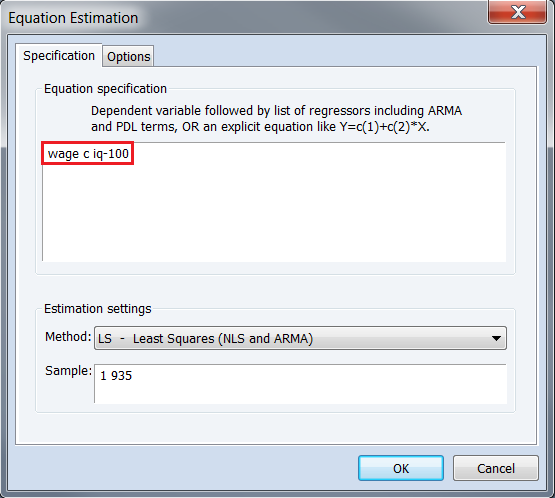
\includegraphics{q3_22}
\end{figure}
\vspace{-\baselineskip}
$$3.\ Name \to Name\ to\ identify\ object: eq02$$
\begin{figure}[H]
	\centering
	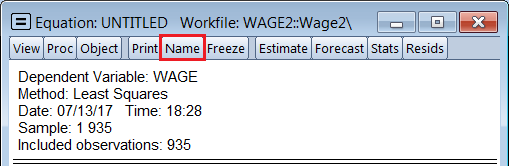
\includegraphics{q3_23}
\end{figure}
\vspace{-\baselineskip}
\begin{figure}[H]
	\centering
	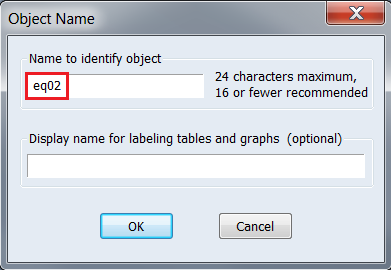
\includegraphics{q3_24}
\end{figure}
\vspace{-\baselineskip}
\noindent To save residuals of this estimated model,
$$eq02 \to Proc \to Make\ Residual\ Series \dots \to Name\ of\ resid\ series: uhat02$$
\begin{figure}[H]
	\centering
	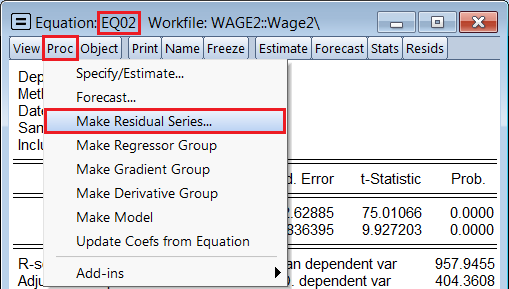
\includegraphics{q3_25}
\end{figure}
\vspace{-\baselineskip}
\begin{figure}[H]
	\centering
	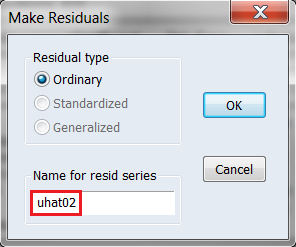
\includegraphics{q3_26}
\end{figure}
\vspace{-\baselineskip}
\noindent After clicking $OK$, the residuals should appears (if not, double-click $uhat02$ from the workfile to see the residuals),
\begin{figure}[H]
	\centering
	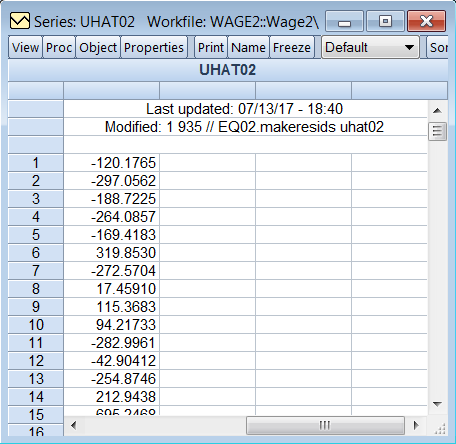
\includegraphics{q3_27}
\end{figure}

%%%%%%%%%% TABLE OBJECT %%%%%%%%%%
\begin{table}[!htbp]
	\centering
	\begin{tabular}{lrrrr}
		\multicolumn{3}{l}{Dependent Variable: WAGE}&\multicolumn{1}{c}{}&\multicolumn{1}{c}{}\\
		\multicolumn{3}{l}{Method: Least Squares}&\multicolumn{1}{c}{}&\multicolumn{1}{c}{}\\
		\multicolumn{3}{l}{Date: 07/13/17   Time: 18:28}&\multicolumn{1}{c}{}&\multicolumn{1}{c}{}\\
		\multicolumn{2}{l}{Sample: 1 935}&\multicolumn{1}{c}{}&\multicolumn{1}{c}{}&\multicolumn{1}{c}{}\\
		\multicolumn{3}{l}{Included observations: 935}&\multicolumn{1}{c}{}&\multicolumn{1}{c}{}\\
		[4.5pt] \hline \\ [-4.5pt]
		\multicolumn{1}{c}{Variable}&\multicolumn{1}{r}{Coefficient}&\multicolumn{1}{r}{Std. Error}&\multicolumn{1}{r}{t-Statistic}&\multicolumn{1}{r}{Prob.}\\
		[4.5pt] \hline \\ [-4.5pt]
		\multicolumn{1}{c}{C}&\multicolumn{1}{r}{$947.2980$}&\multicolumn{1}{r}{$12.62885$}&\multicolumn{1}{r}{$75.01066$}&\multicolumn{1}{r}{$0.0000$}\\
		\multicolumn{1}{c}{IQ-100}&\multicolumn{1}{r}{$8.303064$}&\multicolumn{1}{r}{$0.836395$}&\multicolumn{1}{r}{$9.927203$}&\multicolumn{1}{r}{$0.0000$}\\
		[4.5pt] \hline \\ [-4.5pt]
		\multicolumn{1}{l}{R-squared}&\multicolumn{1}{r}{$0.095535$}&\multicolumn{2}{l}{Mean dependent var}&\multicolumn{1}{r}{$957.9455$}\\
		\multicolumn{1}{l}{Adjusted R-squared}&\multicolumn{1}{r}{$0.094566$}&\multicolumn{2}{l}{S.D. dependent var}&\multicolumn{1}{r}{$404.3608$}\\
		\multicolumn{1}{l}{S.E. of regression}&\multicolumn{1}{r}{$384.7667$}&\multicolumn{2}{l}{Akaike info criterion}&\multicolumn{1}{r}{$14.74529$}\\
		\multicolumn{1}{l}{Sum squared resid}&\multicolumn{1}{r}{$1.38E+08$}&\multicolumn{2}{l}{Schwarz criterion}&\multicolumn{1}{r}{$14.75564$}\\
		\multicolumn{1}{l}{Log likelihood}&\multicolumn{1}{r}{$-6891.422$}&\multicolumn{2}{l}{Hannan-Quinn criter.}&\multicolumn{1}{r}{$14.74924$}\\
		\multicolumn{1}{l}{F-statistic}&\multicolumn{1}{r}{$98.54936$}&\multicolumn{2}{l}{Durbin-Watson stat}&\multicolumn{1}{r}{$1.802114$}\\
		\multicolumn{1}{l}{Prob(F-statistic)}&\multicolumn{1}{r}{$0.000000$}&\multicolumn{1}{c}{}&\multicolumn{1}{c}{}&\multicolumn{1}{c}{}\\
		[4.5pt] \hline \\ [-4.5pt]
	\end{tabular}
	\caption{Regression output of $wage$ on a constant and $(IQ-100)$}
	\label{tbl:regout2}
\end{table}

\noindent When reporting the estimated model, we must not forget to include a `hat' above the dependent variable and $se(\hat{\beta}_j)$ underneath $\hat{\beta}_j$ in parenthesis,
$$\widehat{wage} = \underset{(12.6289)}{947.2980} + \underset{(0.8364)}{8.3031}(IQ-100)$$
\noindent \underline{Similarities between both estimated models:}
\begin{itemize}
	\item Estimated slope coefficient is the same for both estimated models, $\hat{\beta}_1 = \hat{\alpha}_1 = 8.3031$.
	\item $R^2$ statistic is the same for both estimated models, $R^2_{eq01} = R^2_{eq02} = 0.0955$.
	\item The OLS residuals are the same for both estimated models $(Highlight\ uhat01\ \&\ uhat02 \to Open \to As\ Group)$,
	\begin{figure}[H]
		\centering
		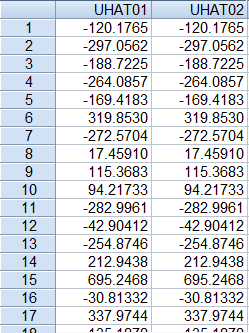
\includegraphics{q3_28}
	\end{figure}
\end{itemize}
\noindent \underline{Differences between both estimated models:}
\begin{itemize}
	\item Estimated intercept coefficient is different for both estimated models, $\hat{\beta}_0 = 116.9916 \neq  \hat{\alpha}_0 = 947.2980$.
	\item Interpretation of estimated intercept of $eq02$, $\hat{\alpha}_0 = 947.2980$, is meaningful: 
	
	\textit{The model predicts that a person with an IQ score of 100 (when IQ-100=0, IQ=100), will earn, on average, \$947.30 per month.}
\end{itemize}
\noindent \textcolor{red}{\underline{(c) What have we learnt?}}

\noindent Subtracting 100 (or any constant) from the independent variable $IQ$ only changes the estimated intercept coefficient. Why?

\noindent Firstly, consider a graph with both regression lines,
$$(Discuss\ in\ class)$$
\vspace{50mm}

\noindent If instead, we subtracted $IQ$ by 1 rather than 100, the regression line will shift to the left by 1 unit (thinking about the data points plotted in a scatter plot which form the first regression line. If these data points take one step to the left, the regression line will also take one step to the left.) so the estimated intercept should increase by 1 unit of the estimated slope i.e. $1\times\hat{\beta}_1$,
$$(Discuss\ in\ class)$$
\vspace{50mm}

\noindent If we now subtract $IQ$ by 100, the regression line shifts to the left by 100 units and estimated intercept should increase by 100 units of the estimated slope i.e $100\times\hat{\beta}_1$,
$$(Discuss\ in\ class)$$
\vspace{50mm}

\newpage
\section*{Question 4}
\noindent \underline{Dummy variables \& linear independence of matrix columns}

\noindent EViews workfile: $wage1tute4.wf1$

\noindent Suppose that each observation in our sample belongs into one of categories, $female$ or $male$. 

\noindent The dummy variable $female$ is binary and equals to 1 if the individual is female and 0 otherwise, 
$$female =  $$

\noindent The dummy variable $male$ is binary and equals to 1 if the individual is male and 0 otherwise, 
$$male =  $$

\noindent Consider a regression of $wage$ on these two dummy variables without a constant,
$$wage = \beta_1female + \beta_2male + u$$

\noindent \textcolor{red}{\ul{(a) Sketch the \textbf{X} matrix for this regression and assume that $n_1$ observations are females, $n_2$ observations are males and that our sample size is given by $n_1+n_2=n$}}

\noindent For cross-sectional data ($wage1tute4.wf1$ contains cross-sectional data), rearranging the order of observations  does not change statistical results.

\noindent For ease of notation, we arrange the first $n_1$ observations to be females and the last $n_2$ observations to be males. This gives us the following \textbf{X} matrix,
\begin{equation*}
\underset{n\times2}{\textbf{X}} = \begin{array}{c@{\!\!\!}l}
\left[ \begin{array}[c]{ccccc}
1 & 0 \\
1 & 0 \\
\vdots & \vdots \\
1 & 0 \\
0 & 1 \\
0 & 1 \\
\vdots & \vdots \\
0 & 1 \\
\end{array}  \right]
&
\begin{array}[c]{@{}l@{\,}l}
\left. \begin{array}{c} \vphantom{0} \\ \vphantom{0} \\\vphantom{\vdots}\\ \vphantom{0} \end{array} \right\} & \text{$n_1$} \\
\left. \begin{array}{c} \vphantom{1} \\ \vphantom{1} \\ \vphantom{\vdots}
\\ \vphantom{1}  \end{array} \right\} & \text{$n_2$} \\
\end{array}
\end{array}
\end{equation*}
\noindent The $1^{st}$ and $2^{nd}$ column of the \textbf{X} matrix represents the $female$ and $male$ dummy variable respectively.

\newpage
\noindent \textcolor{red}{Are the columns of \textbf{X} linearly independent?}
\justify
\begin{blueframed}
	\textcolor{blue}{\textbf{Background}}
	\vspace{-\baselineskip}
	\justify
	\textcolor{blue}{\underline{Linear independence of columns of matrix}}
	
	\noindent \textcolor{blue}
	{
		The columns of a matrix are linearly independent if the linear combination of the columns of the matrix equals to 0 only when each column is weight (multiplied) by 0. (Another way to think about this is if the columns of a matrix can form a linearly dependent set, then the columns of the matrix are linearly dependent.)
	}
	
	\noindent \textcolor{blue}
	{
		If we denote the $1^{st}$, $2^{nd}$ through to the $r^{th}$ column of matrix \textit{\textbf{X}} as, $\textit{\textbf{x}}_\textbf{1}$, $\textit{\textbf{x}}_\textbf{2}$ and $\textit{\textbf{x}}_\textbf{r}$ respectively, then the columns of \textbf{X} will be linearly independent if,
		$$ 
		\textit{\textbf{x}}_\textbf{1}a_1 + \textit{\textbf{x}}_\textbf{2}a_2 + \dots + \textit{\textbf{x}}_\textbf{r}a_r = 0
		$$
		$$
		\underline{only\ when}
		$$
		$$
		a_1 = a_2 = \dots = a_r = 0
		$$ If the columns of \textbf{X} are not linearly independent, then $\textbf{X}'\textbf{X}$ will not be invertible,
		\sout{$(\textbf{X}'\textbf{X})^{-1}$}
		and the OLS estimator,
		$$
		\widehat{\boldsymbol{\beta}} 
		= (\textbf{X}'\textbf{X})^{-1}\textbf{X}'\textbf{y}
		$$
		cannot be computed.
	}
\end{blueframed}
\noindent Since the linear combination of the columns of \textbf{X} equals to 0 only when each column is weighted (multiplied) by 0,
$$
\begin{bmatrix}
1 \\
1 \\
\vdots \\
1 \\
0 \\
0 \\
\vdots \\
0
\end{bmatrix}
a_1
+
\begin{bmatrix}
0 \\
0 \\
\vdots \\
0 \\
1 \\
1 \\
\vdots \\
1
\end{bmatrix}
a_2
=
0
\qquad
\underline{only\ when}\ a_1 = a_2 = 0
$$
\noindent the columns of \textbf{X} are linearly independent $\therefore$ the OLS estimator can be calculated.

\newpage
\noindent \textcolor{red}
{(b) Use the OLS formula $\widehat{\boldsymbol{\beta}} 
	= (\textbf{X}'\textbf{X})^{-1}\textbf{X}'\textbf{y}$ and derive the OLS estimator in this case.}

\noindent Let $y = wage$
\begin{align*}
\textit{\textbf{X}}'\textit{\textbf{X}}
&=
\begin{spmatrix}{2 \times n}
1 & 1 & \cdots & 1 & 0 & 0 & \cdots & 0 \\
0 & 0 & \cdots & 0 & 1 & 1 & \cdots & 1
\end{spmatrix}
\begin{spmatrix}{n \times 2}
1 & 0 \\
1 & 0 \\
\vdots & \vdots \\
1 & 0\\
0 & 1 \\
0 & 1 \\
\vdots & \vdots \\
0 & 1
\end{spmatrix}
=
\begin{bmatrix}
\sum_{i=1}^{n_1}1 & 0 \\
0 & \sum_{i=1}^{n_2}1
\end{bmatrix}
=
\begin{bmatrix}
n_1 & 0 \\
0 & n_2
\end{bmatrix} \\
\therefore{}(\textit{\textbf{X}}'\textit{\textbf{X}})^{-1}
&=
\begin{bmatrix}
\dfrac{1}{n_1} & 0 \\
0 & \dfrac{1}{n_2}
\end{bmatrix} \\ \\
(for\ the\ &inverse\ of\ a\ diagonal\ matrix,\ simply\ take\ inverse\ of\ diagonal\ elements) \\
\\
\textit{\textbf{X}}'\textit{\textbf{y}}
&=
\begin{spmatrix}{2 \times n}
1 & 1 & \cdots & 1 & 0 & 0 & \cdots & 0 \\
0 & 0 & \cdots & 0 & 1 & 1 & \cdots & 1
\end{spmatrix}
\begin{spmatrix}{n \times 1}
y_1 \\
y_2 \\
\vdots \\
y_{n_1} \\
y_{n_{1} + 1} \\
y_{n_{1} + 2} \\
\vdots \\
y_{n_{1} + n_{2}} 
\end{spmatrix}
=
\begin{spmatrix}{2 \times 1}
y_1 + y_2 + \dots + y_{n_1} \\
y_{n_{1} + 1} +y_{n_{1} + 2} + \dots + y_{n_{1} + n_{2}}
\end{spmatrix} \\
&=
\begin{bmatrix}
\sum_{i=1}^{n_1} y_i \\
\sum_{i=n_{1} + 1}^{n_{1} + n_{2}} y_i
\end{bmatrix}\\
\therefore{}\widehat{\boldsymbol{\beta}} 
&= (\textit{\textbf{X}}'\textit{\textbf{X}})^{-1}\textit{\textbf{X}}'\textit{\textbf{y}}
=
\begin{bmatrix}
\dfrac{1}{n_1} & 0 \\
0 & \dfrac{1}{n_2}
\end{bmatrix} 
\begin{bmatrix}
\sum_{i=1}^{n_1} y_i \\
\sum_{i=n_{1} + 1}^{n_{1} + n_{2}} y_i
\end{bmatrix}
=
\begin{bmatrix}
\dfrac{1}{n_1} \times \sum_{i=1}^{n_1} y_i + 0 \times \sum_{i=n_{1} + 1}^{n_{1} + n_{2}} y_i \\
0 \times \sum_{i=1}^{n_1} y_i + \dfrac{1}{n_2} \times \sum_{i=n_{1} + 1}^{n_{1} + n_{2}} y_i
\end{bmatrix} \\
&=
\begin{bmatrix}
\dfrac{1}{n_1}\sum_{i=1}^{n_1} y_i \\
\dfrac{1}{n_2}\sum_{i=n_{1} + 1}^{n_{1} + n_{2}} y_i
\end{bmatrix}
=
\begin{bmatrix}
\overline{y}_{female} \\
\overline{y}_{male}
\end{bmatrix}
=
\begin{bmatrix}
\overline{wage}_{female} \\
\overline{wage}_{male}
\end{bmatrix}
\end{align*}

\newpage
\noindent \textcolor{red}{Comment on the result.}

\noindent We find that by regressing the dependent variable on dummy variables without a constant term, the OLS estimator is the sample mean of the dependent variable for each group,
$$
\widehat{\boldsymbol{\beta}}
=
\begin{bmatrix}
\hat{\beta}_1 \\
\hat{\beta}_2
\end{bmatrix}
=
\begin{bmatrix}
\overline{y}_{female} \\
\overline{y}_{male}
\end{bmatrix}
$$

\noindent \textcolor{red}{Verify results by creating the dummy variable $male$ in $wage1tute3.wf1$ and running a regression of $wage$ on $female$ and $male$ without a constant.}
$$
wage = \beta_1female + \beta_2male + u
$$
\noindent $wage1tute3.wf1$ contains the $female$ dummy variable, 
\begin{figure}[H]
	\centering
	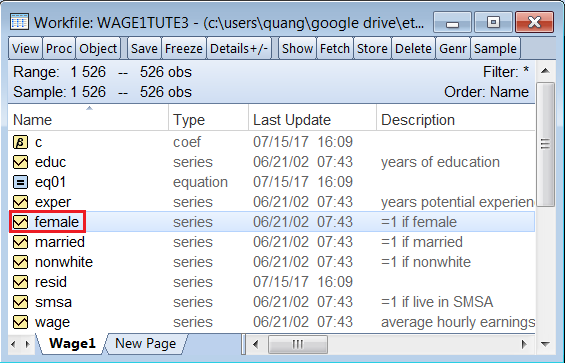
\includegraphics{q2_1}
\end{figure}
\vspace{-\baselineskip}
\begin{figure}[H]
	\centering
	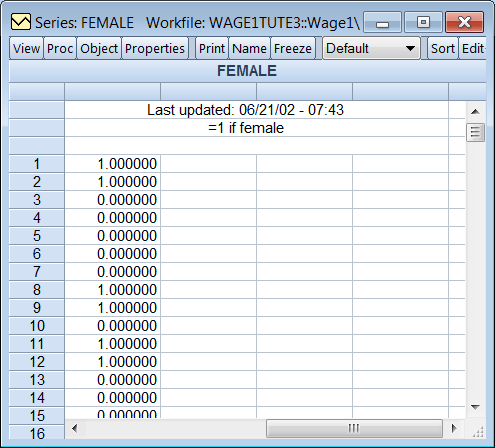
\includegraphics{q2_2}
\end{figure}
\vspace{-\baselineskip}
\noindent Since the $male$ dummy variable is a function of the $female$ dummy variable,
$$
male_i = 1-female_i \qquad i = 1,2,\dots,n
$$
\noindent To create the $male$ dummy variable in EViews,
$$Quick \to Generate\ Series$$
\begin{figure}[H]
	\centering
	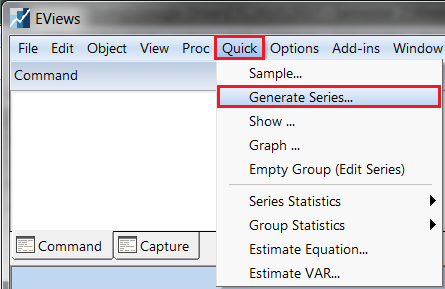
\includegraphics{q2_3}
\end{figure}
\vspace{-\baselineskip}
$$Enter\ Equation: male=1-female$$
\begin{figure}[H]
	\centering
	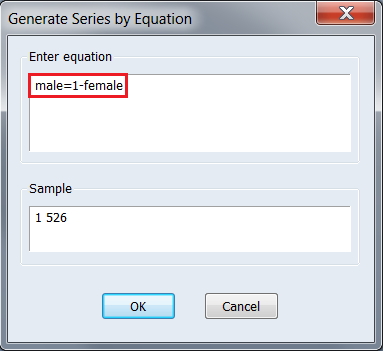
\includegraphics{q2_4}
\end{figure}
\vspace{-\baselineskip}
\noindent To estimate $wage$ on $female$ and $male$ without a constant, 
$$wage = \beta_1female +\beta_2male + u$$
$$Quick \to Estimate\ Equation$$
\begin{figure}[H]
	\centering
	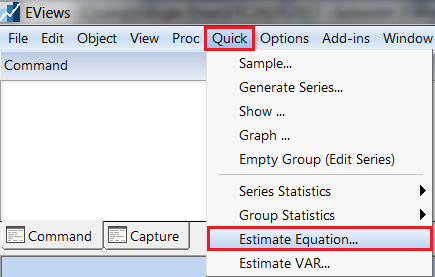
\includegraphics{q1_2}
\end{figure}
\vspace{-\baselineskip}
$$Equation\ Estimation: wage\ female\ male$$
\begin{figure}[H]
	\centering
	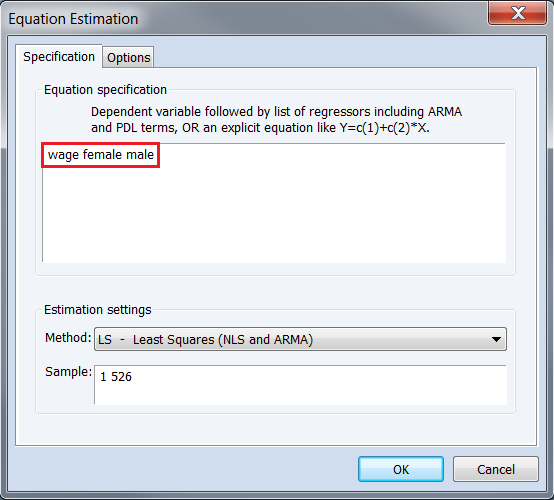
\includegraphics{q2_5}
\end{figure}
\vspace{-\baselineskip}
%%%%%%%%%% TABLE OBJECT %%%%%%%%%%
\begin{table}[H]
	\centering
	\begin{tabular}{lrrrr}
		\multicolumn{3}{l}{Dependent Variable: WAGE}&\multicolumn{1}{c}{}&\multicolumn{1}{c}{}\\
		\multicolumn{3}{l}{Method: Least Squares}&\multicolumn{1}{c}{}&\multicolumn{1}{c}{}\\
		\multicolumn{3}{l}{Date: 07/16/17   Time: 17:08}&\multicolumn{1}{c}{}&\multicolumn{1}{c}{}\\
		\multicolumn{2}{l}{Sample: 1 526}&\multicolumn{1}{c}{}&\multicolumn{1}{c}{}&\multicolumn{1}{c}{}\\
		\multicolumn{3}{l}{Included observations: 526}&\multicolumn{1}{c}{}&\multicolumn{1}{c}{}\\
		[4.5pt] \hline \\ [-4.5pt]
		\multicolumn{1}{c}{Variable}&\multicolumn{1}{r}{Coefficient}&\multicolumn{1}{r}{Std. Error}&\multicolumn{1}{r}{t-Statistic}&\multicolumn{1}{r}{Prob.}\\
		[4.5pt] \hline \\ [-4.5pt]
		\multicolumn{1}{c}{FEMALE}&\multicolumn{1}{r}{$4.587659$}&\multicolumn{1}{r}{$0.218983$}&\multicolumn{1}{r}{$20.94980$}&\multicolumn{1}{r}{$0.0000$}\\
		\multicolumn{1}{c}{MALE}&\multicolumn{1}{r}{$7.099489$}&\multicolumn{1}{r}{$0.210008$}&\multicolumn{1}{r}{$33.80578$}&\multicolumn{1}{r}{$0.0000$}\\
		[4.5pt] \hline \\ [-4.5pt]
		\multicolumn{1}{l}{R-squared}&\multicolumn{1}{r}{$0.115667$}&\multicolumn{2}{l}{Mean dependent var}&\multicolumn{1}{r}{$5.896103$}\\
		\multicolumn{1}{l}{Adjusted R-squared}&\multicolumn{1}{r}{$0.113979$}&\multicolumn{2}{l}{S.D. dependent var}&\multicolumn{1}{r}{$3.693086$}\\
		\multicolumn{1}{l}{S.E. of regression}&\multicolumn{1}{r}{$3.476254$}&\multicolumn{2}{l}{Akaike info criterion}&\multicolumn{1}{r}{$5.333582$}\\
		\multicolumn{1}{l}{Sum squared resid}&\multicolumn{1}{r}{$6332.194$}&\multicolumn{2}{l}{Schwarz criterion}&\multicolumn{1}{r}{$5.349800$}\\
		\multicolumn{1}{l}{Log likelihood}&\multicolumn{1}{r}{$-1400.732$}&\multicolumn{2}{l}{Hannan-Quinn criter.}&\multicolumn{1}{r}{$5.339932$}\\
		\multicolumn{1}{l}{Durbin-Watson stat}&\multicolumn{1}{r}{$1.817601$}&\multicolumn{1}{c}{}&\multicolumn{1}{c}{}&\multicolumn{1}{c}{}\\
		[4.5pt] \hline \\ [-4.5pt]
	\end{tabular}
	\caption{Regression output of $wage$ on $female$ and $male$}
	\label{tbl:regout2}
\end{table}

\vspace{-\baselineskip}
\noindent When reporting the estimated model, we must not forget to include a `hat' above the dependent variable and $se(\hat{\beta}_j)$ underneath $\hat{\beta}_j$ in parenthesis,
$$\widehat{wage} = \underset{(0.2190)}{4.5877}female + \underset{(0.2100)}{7.0995}male$$
\noindent To obtain the sample mean of $wage$ for females and males in EViews,
$$\overline{wage}_{female} = ?$$
$$\overline{wage}_{male} = ?$$
$$Double\ click\ on\ wage \to View \to Descriptive\ Stats\ \&\ Tests \to Stats\ by\ Classification$$
\begin{figure}[H]
	\centering
	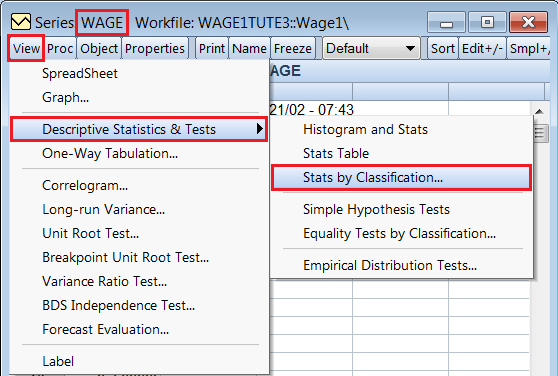
\includegraphics{q2_6}
\end{figure}
\vspace{-\baselineskip}
$$Series/Group\ for\ classify: female$$
\begin{figure}[H]
	\centering
	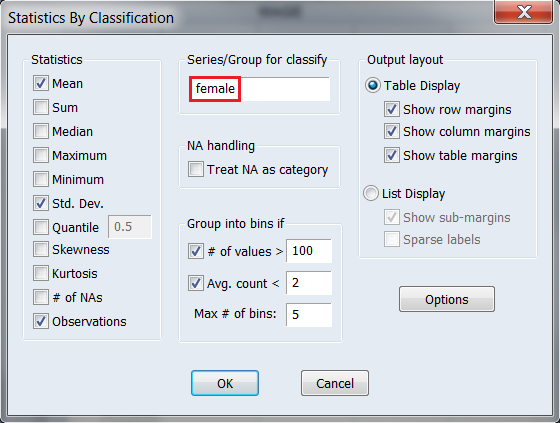
\includegraphics{q2_7}
\end{figure}
\vspace{-\baselineskip}
%%%%%%%%%% TABLE OBJECT %%%%%%%%%%
\begin{table}[H]
	\centering
	\begin{tabular}{lrrr}
		\multicolumn{4}{l}{Descriptive Statistics for WAGE}\\
		\multicolumn{4}{l}{Categorized by values of FEMALE}\\
		\multicolumn{3}{l}{Date: 07/16/17   Time: 17:34}&\multicolumn{1}{c}{}\\
		\multicolumn{2}{l}{Sample: 1 526}&\multicolumn{1}{c}{}&\multicolumn{1}{c}{}\\
		\multicolumn{3}{l}{Included observations: 526}&\multicolumn{1}{c}{}\\
		[4.5pt] \hline \\ [-4.5pt]
		\multicolumn{1}{c|}{FEMALE}&\multicolumn{1}{r}{Mean}&\multicolumn{1}{r}{Std. Dev.}&\multicolumn{1}{r}{Obs.}\\
		\multicolumn{1}{c|}{0}&\multicolumn{1}{r}{$7.099489$}&\multicolumn{1}{r}{$4.160858$}&\multicolumn{1}{r}{$274$}\\
		\multicolumn{1}{c|}{1}&\multicolumn{1}{r}{$4.587659$}&\multicolumn{1}{r}{$2.529363$}&\multicolumn{1}{r}{$252$}\\
		\multicolumn{1}{c|}{All}&\multicolumn{1}{r}{$5.896103$}&\multicolumn{1}{r}{$3.693086$}&\multicolumn{1}{r}{$526$}\\
		[4.5pt] \hline \\ [-4.5pt]
	\end{tabular}
	\caption{Sample mean and standard deviation of female and male $wage$}
	%\label{tab:}
\end{table} \vspace{-\baselineskip} \begin{align*} 
	\overline{wage}_{female} &= 4.5877 = \hat{\beta}_1 \\
	\overline{wage}_{male} &= 7.0995 = \hat{\beta}_2
\end{align*} 

\newpage
\noindent \textcolor{red}
{
	\ul{(c) Suppose we have a constant in addition to the two dummy variables $female$ and $male$.}
}

\noindent \textcolor{red}
{
	Write down the \textit{\textbf{X}} matrix for this case.
}
\begin{equation*}
\underset{n\times3}{\textit{\textbf{X}}} = \begin{array}{c@{\!\!\!}l}
\left[ \begin{array}[c]{ccccc}
1 & 1 & 0 \\
1 & 1 & 0 \\
\vdots & \vdots & \vdots \\
1 & 1 & 0 \\
1 & 0 & 1 \\
1 & 0 & 1 \\
\vdots & \vdots & \vdots \\
1 & 0 & 1 \\
\end{array}  \right]
&
\begin{array}[c]{@{}l@{\,}l}
\left. \begin{array}{c} \vphantom{0} \\ \vphantom{0} \\\vphantom{\vdots}\\ \vphantom{0} \end{array} \right\} & \text{$n_1$} \\
\left. \begin{array}{c} \vphantom{1} \\ \vphantom{1} \\ \vphantom{\vdots}
\\ \vphantom{1}  \end{array} \right\} & \text{$n_2$} \\
\end{array}
\end{array}
\end{equation*}
\noindent \textcolor{red}
{
	Are the columns of \textit{\textbf{X}} linearly independent?
}

\noindent The columns of \textit{\textbf{X}} will be linearly independent if,
$$
\begin{bmatrix}
1 \\
1 \\
\vdots \\
1 \\
1 \\
1 \\
\vdots \\
1
\end{bmatrix}
a_1
+
\begin{bmatrix}
1 \\
1 \\
\vdots \\
1 \\
0 \\
0 \\
\vdots \\
0
\end{bmatrix}
a_2
+
\begin{bmatrix}
0 \\
0 \\
\vdots \\
0 \\
1 \\
1 \\
\vdots \\
1
\end{bmatrix}
a_3
=
0
\qquad
\underline{only\ when}\ a_1 = a_2 = a_3 = 0
$$
\noindent However, there are linear combinations of the columns of \textit{\textbf{X}} that equal to 0 when $a_1 \ne 0, a_2 \ne 0, a_3 \ne 0$. For example, when, $a_1=1,a_2=-1$ and $a_3=-1$
$$
\begin{bmatrix}
1 \\
1 \\
\vdots \\
1 \\
1 \\
1 \\
\vdots \\
1
\end{bmatrix}
-
\begin{bmatrix}
1 \\
1 \\
\vdots \\
1 \\
0 \\
0 \\
\vdots \\
0
\end{bmatrix}
-
\begin{bmatrix}
0 \\
0 \\
\vdots \\
0 \\
1 \\
1 \\
\vdots \\
1
\end{bmatrix}
=
0
\qquad
a_1 = 1, a_2 = -1, a_3 = -1
$$
\noindent Therefore, the columns of \textit{\textbf{X}} are not linearly independent. This implies that $\textit{\textbf{X}}'\textit{\textbf{X}}$ will not be invertible so the OLS estimator cannot be computed. This is also called a problem of \underline{perfect collinearity} i.e. an exact linear relationship among the independent variables.

\noindent \textcolor{red}
{
	What is the dimension of the column space of \textit{\textbf{X}}?
}

\noindent Consider an example in which we have only 3 rows in our \textit{\textbf{X}} matrix (3 observations in our sample) and let the first 2 observations be female and the last observation be male,
$$
\underset{3\times3}{\textit{\textbf{X}}}
=
\begin{bmatrix}
1 & 1 & 0\\
1 & 1 & 0\\
1 & 0 & 1
\end{bmatrix}
$$
$$(2\ females\ and\ 1\ male)$$
\noindent Each column of the \textit{\textbf{X}} matrix plotted on a 3-dimensional $(x,y,z)$ axes, would be vectors pointed to the coordinates,
$$(1,1,1)$$
$$(1,1,0)$$
$$(0,0,1)$$
\noindent from the origin.

\noindent Since the column space of a matrix is characterised by the columns of the matrix, we find that although we have 3 columns, it only forms a 2-dimensional column space. All 3 column vectors lie on this column space, but we only need 2 columns and not 3 (it can be any 2 of the 3 columns) to obtain this column space i.e. one of the columns is redundant given the other two.

\noindent \textcolor{red}
{
	If a regression has a constant, only add one dummy variable for an attribute that has two categories (such as male, female). Explain.
}

\noindent For a regression with a constant, we cannot include both the $female$ AND $male$ dummy variable because it will cause the columns of the matrix to be linearly dependent (problem of perfect collinearity) and $\textit{\textbf{X}}'\textit{\textbf{X}}$ will not be invertible, so the OLS estimator, 
$$
\widehat{\boldsymbol{\beta}} 
= (\textit{\textbf{X}}'\textit{\textbf{X}})^{-1}\textit{\textbf{X}}'\textit{\textbf{y}}
$$
\noindent cannot be computed.





\end{document}
